\label{KonzepteinverseProbleme}

\section{Konzepte zum Lösen inverser Probleme}

In den letzen drei Kapiteln (Vorlesungswochen) haben wir einen Einblick in die
Vorgehensweise der Maximum-Likelihood-Methode erhalten:
\begin{enumerate}
\item Die Idee von \textsl{Modell} und \textsl{Lösen inverser Probleme} wurde
  genannt.
\item Zur Lösung inverser Probleme wurde das Schätzen von Parametern, die
 linear in die Modellgleichung eingehen, durch \textsl{lineare Regression} vorgestellt.
\item Ein Einblick in mögliche Verfahren zur Lösung inverser Probleme durch
  Schätzen von Parametern, die nicht-linear in die Modellgleichung eingehen,
  wurde gegeben. Hier wurden kurz drei Verfahren zur \textsl{nicht-linearen Optimierung}
  vorgestellt.
\end{enumerate}
Wir haben dabei gesehen, dass es bei der Messdatenanalyse um die Schätzung von
physikalischen Größen geht, die indirekt über das Messen anderer Größen,
direkter Messgrößen, ermittelt werden.
Die Aufgabe der Messtechnik lässt sich auch beschreiben als die Bestimmung
des Wertes von physikalischen Größen durch Messverfahren, die auf
physikalischen Prinzipien basieren. Die von einem Sensorsystem angezeigten
Größen sind dabei im allgemeinem andere Größen als diejenigen, die zu messen sind.

Wir hatten in der ersten Vorlesung, in Abschnitt \ref{ModelleStatistik},
das Beispiel \glqq Beugung am Gitter\grqq ~betrachtet,
um die Aufgabenstellung zu verstehen, dass man
aus den einem Messsystem direkt zugänglichen Größen die gesuchten physikalischen
Größen gewinnen möchte. Dabei wurde der Begriff des \textsl{Lösens inverser Probleme}
eingeführt. Nachdem wir bereits Methoden zur Ermittlung von indirekten
Messgrößen als Modellparameter kennen gelernt haben, haben wir die Chance uns
unter den Ideen dieses Konzeptes mehr vorstellen zu können.

Darüber hinaus wurde in Abschnitt \ref{ModelleStatistik} schon mal erwähnt, dass
es etwas unterschiedliche Konzepte oder Heransgehensweisen für Schätzverfahren gibt.
Auf der einen Seite steht der sogenannte \textsl{frequentistische} Ansatz, bei dem allein
Beobachtungswerte direkter Größen verwendet werden und die Annahmen über die
Verteilung der Streuung der direkten Größen impliziet schon ins Schätzverfahren
selber eingebaut sind. Der Begriff Frequenz wurde an dieser Stelle aus der
englischen Sprachkonvention \textsl{frequency} übernommen. Das
heißt hier \textsl{Häufigkeit} und nicht \textsl{Frequenz} wie wir das im Deutschen
vielfach mit einer periodischen Bewegung verbunden verstehen. Aber auch die
deutsche Sprache kennt die Sprechweise: \glqq Dies oder jenes Restaurant oder so
wird gut frequentiert\grqq ~im Sinne von \glqq wird häufig besucht\grqq.

Eine Verallgemeinerung der Schätzmethoden wurde in den letzten Jahrzehnten
in die Messdatenanalyse eingeführt, bei der auch die Modellparameter selber als
Zufallsgrößen behandelt werden. Auch ihnen wird eine Streuung, also
Wahrscheinlichkeitsverteilung zugrunde gelegt. Bei diesen Verfahren lassen sich
Schätzwerte und Werte zur Unsicherheit der Modellparameter in die aktuelle
Schätzung mit einbeziehen. Diese verallgemeinerten Methoden, die die Modellparameter
als Zufallsgrößen betrachten, werden \textsl{bayesische} Methoden genannt.

Bevor wir diese beiden Ansätze (frequentistisch und bayesisch) gegenüber
stellen und vergleichen, wollen wir folgende
zwei Blickrichtungen, messtechnische Aufgaben zu betrachten, beleuchten:
\begin{itemize}
\item als Modell von der Physik des Messprinzips gemeinsam mit dem statistischen
Modell, dass die Größen Zufallsgrößen sind,
\item als inverses Problem.
\end{itemize}
Ein Modell wird dargestellt durch eine Vorstellung darüber, wie die
indirekten Messgrößen $Y_m$ mit den direkten Messgrößen $X_i$ verknüpft sind:
\begin{equation}
(Y_1, \dots, Y_M) \xrightarrow{\mathrm{Modell}} (X_1, \dots, X_N)
\label{forwardModel1}
\end{equation}
\begin{figure}
\begin{center}
\includegraphics[width=0.8\textwidth, angle = 0]{04_vorlesung/media/Modell1.pdf}
\end{center}
\caption{Modellbildung zur Gewinnung indirekter Messgrößen aus direkten Messgrößen}
\end{figure}

Ein Messvorgang liefert Beobachtungen zu den direkten Messgrößen.
Die wahren Werte der indirekten Größen bleiben verborgen. Die
indirekten Größen können nur geschätzt werden, oftmals auch nur approximiert werden,
weil die Modelle den physikalischen Sachverhalt nur annähernd beschreiben;
denn die Realität ist deutlich komplexer und wird von vielfältigen Einflussfaktoren
bestimmt. Die approximierenden und zufällig streuenden Größen, die die indirekten Messgrößen
repräsentieren, sind die Modellparameter.
Die Abweichungen der Modellparameter entstehen also zum einen
durch vereinfachende Modellannahmen und zum anderen durch zufällige Einflüsse wie das
thermische Rauschen von Elektronik oder Vibrationen im Laborraum.

Im vorigen Kapitel hatten wir bereits den Bezeichner $\mathbf{p}$ für die Modellparameter
verwendet: $\mathbf{p} = (P_1, \dots, P_M)$.
Der Buchstabe $\mathbf{p}$ steht hier einfach nur für den Anfangbuchstaben
von dem Begriff Parameter und der Fettdruck weist darauf hin, dass es ein Vektor mit vielen
Einzelparametern sein kann und dient ferner dazu, das Symbol von dem für die Wahrscheinlichkeitsdichte
zu unterscheiden. Diese wird mit $p$ für den Anfangsbuchstaben von \textsl{probability} bezeichnet.
Für die einzelnen Parameter $P_m$ verwenden wir hier den Großbuchstaben, um die Unterscheidung zur
Wahrscheinlichkeitsdichtefunktion zu haben, sowie in Anlehnung an die Konvention Großbuchstaben
$X_i$ und $Y_m$ für die Messgrößen zu verwenden.
\begin{equation}
P_1 \approx Y_1, \dots, P_M \approx Y_M
\end{equation}
Der Schätzvorgang wird als \textsl{Lösen eines inversen Problems} interpretiert.
\begin{equation}
(X_1, \dots, X_N) \xrightarrow{\mathrm{inverses \; Problem}} (Y_1, \dots, Y_M)
\label{inverseProblemEq}
\end{equation}

Dazu haben wir die \textsl{Maximum-Likelihood}-Methode kennen gelernt, und gesehen, wie
aus ihr die Methode der kleinsten Residuenquadratsumme hervorgeht. Die Wahrscheinlichkeit,
dass ein Messwert um den Wert $\varepsilon$ von dem geschätzten Modell abweicht, folgt
einer Normalverteilung. Mit anderen Worten kann man auch sagen, dass
die Verteilung der Residuen eine Gaußverteilung ist.
Die Begriffe Gaußverteilung und Normalverteilung verwenden wir synonym.
\begin{equation}
p(\varepsilon | \theta_1,\dots,\theta_M, \sigma) \; = \; \frac{1}{\sigma \sqrt{2 \pi}}
e^{-\frac{1}{2} \left(\frac{\varepsilon}{\sigma}\right)^2}
\label{Maximumlikelihood1}
\end{equation}
Die Symbolik $p(\varepsilon | \theta_1,\dots,\theta_M, \sigma)$ wird gesprochen:
\begin{quote}
Wahrscheinlichkeit $p$ des Eintretens des Ereignises $\varepsilon$
gegeben die Parameter $\theta_1,\dots,\theta_M$ und $\sigma$.
\end{quote}
Der Sprachgebrauch \glqq Eintretens des Ereignisses $\varepsilon$\grqq ~stellt die
Sprechweise der Statistik für \textsl{bedingte Wahrscheinlichkeiten} dar.

\textsl{Bedingte Wahrscheinlichkeit} heißt:
\begin{quote}
Die Wahrscheinlichkeit des Eintretens
zweier Ereignisse $A_1$ und $A_2$ geteilt durch die Wahrscheinlichkeit des Eintretens von $p(A_2)$
\begin{equation}
p(A_1 | A_2) \; = \; \frac{p(A_1 \; \mathrm{und} \; A_2)}{p(A_2)}
\end{equation}
\end{quote}
Zur Illustration des Begriffs der bedingten Wahrscheinlichkeit betrachten wir ein
Kartendeck mit 52 Spielkarten: Die Anzahl der Buben $B$ ist $4$, die Wahscheinlichkeit, einen Buben
zu ziehen, ist $4/52$, die
Wahrscheinlichkeit $p(B | F)$ von allen Bildern bzw.\ Figuren $F = \{B, D, K\}$, einen
 Buben zu ziehen, ist $p(B | F) = 1/3$, die Wahrscheinlichkeit, eine Bildkarte zu ziehen ist $12/52$
$$
p(B | F) = \frac{p(B)}{p(F)} = \frac{4/52}{12/52} = \frac{4}{12} = \frac{1}{3} .
$$

In den angewandten Wissenschaften, Messtechnik,
Elektrotechnik, etc.\ spricht man von der Wahrscheinlichkeit, dass die Messgröße
oder hier die Abweichung der Messgröße vom Modell einen Wert $\varepsilon$ annimmt oder
dass dieser Wert \glqq beobachtet\grqq ~wird unter der Bedingung, dass die Modellparameter
die Werte $\theta_1,\dots,\theta_M, \sigma$ haben.


In Kapitel \ref{KapitellinReg} wurden Sie mit der Regressionsrechnung vertraut gemacht, die
eine spezielle Anwendung der Maximum-Likelihood-Methode darstellt, bei der
Größen beteiligt sind, die keine Zufallsgrößen darstellen, die Regressoren.
Die Residuen und entsprechend die Regressanden sind die Zufallsgrößen,
für die die in Gl.~(\ref{Maximumlikelihood1}) formulierte Wahrscheinlichkeitsdichte
angenommen wird.
Diese Modellannahme, dass die \textsl{Residuen} normalverteilt seien,
hatten wir in Abschnitt \ref{RegressionsIdee} wie folgt formuliert:
\begin{quote}
Die abhängigen Größen $Y$, d.h.\ die \textsl{Regressanden}, streuen und ihre Residuen sind
	normalverteilt mit Erwartungswert $E(\varepsilon) = 0$ und Varianz $\mathrm{Var}(\varepsilon) = \sigma^2$.
	Die Residuen sind \textsl{unabhängig und identisch verteilt}, kurz u.i.v.
	\begin{equation}
	\varepsilon \; \overset{\mathrm{u.i.v.}}{\sim} \; \mathcal{N}(0,\sigma) .
	\end{equation}
\end{quote}
Ein Residuum der linearen Regression mit $Y$ als Regressand und $X_i$ als Regressoren
hat folgende Gestalt
\begin{equation}
\varepsilon_j \; = \; Y_j \; - \; \sum\limits_{i=1}^{M} \theta_i \, X_{i,j}
\end{equation}
wobei der Bezeichner $Y$ der Regressionsrechnung die direkte Messgröße ist und die
Regressoren ebenfalls zu den direkten Größen gehören, jedoch nicht als Zufallsgrößen mit
Streuung, sondern mit vorgegebenen, deterministischen Werten.

Ein Residuum nach der Methode der kleinsten Quadrate für ein Modell mit genau nur einer
einzigen Zufallsgröße $X$ mit einem Modellparameter $\mu$ ist einfach
\begin{equation}
\varepsilon_j \; = \; X_j \, - \, \mu .
\label{oneQuantityOnly1}
\end{equation}

Im Fall der linearen Regression repäsentiert $\mathbf{p} = (\theta_1,\dots,\theta_M)$,
im Fall der Geraden $\mathbf{p} = (\alpha, d)$ und im Fall der Einzelgröße
$\mathbf{p} = \mu$.

Die Schätzung von Modellparametern besteht dann darin, die Modellparameter auszuprobieren,
d.h.\ viele unterschiedliche Werte \glqq auszuprobieren\grqq,
\begin{equation}
(P_1, \dots, P_M) \xrightarrow{\mathrm{Modell}} (X_{\mathrm{Modell},1,j}, \dots, X_{\mathrm{Modell},N,j})
\label{forwardModel2}
\end{equation}
 und das Ergebnis der
Modellrechnungen (\ref{forwardModel2}) mit den beobachteten Werten zu vergleichen, solange,
bis das Ergebnis \glqq gut zu den beobachteten Werten passt\grqq.

%, die Kostenfunktion minimal wird.

%Dieses Ausprobieren, d.h.\ die Variation bzw.\ iterative Veränderung der Modellparameter
%kann beispielsweise dadurch realisiert werden, dass die Steigung der Kostenfunktion,
%d.h.\ die Gradientenfunktion $\nabla Q$, berechnet wird und zu jedem Iterationsschritt der
%entsprechende Parametervektor eingesetzt, um den Schrittvektor zum nächsten Iterationsschritt
%zu erhalten. Einen Einblick, wie numerische
%Optimierungsverfahren prinzipiell funktionieren können, haben wir im vorigen Kapitel erhalten.

Die beiden Annahmen, dass - wie wir in Kapitel \ref{KapitellinReg} bereits bei der linearen Regression
aufgeschrieben hatten - jede einzelne Beobachtung unabhängig und identisch verteilt
(u.i.v) ist, sind Voraussetzung der Maximum-Likelihood-Methode:
\begin{itemize}
\item Jeder Messpunkt wurde unabhängig von allen anderen gewonnen.
\item Jeder Messpunkt ist identisch verteilt (sie haben die gleiche Streuung).
\end{itemize}

Die gemeinsame Wahrscheinlichkeitsdichte, engl.\ \textsl{joint probability density}, der
Residuen von $j$ voneinander unabhängigen Messungen ist dann das Produkt der
Wahrscheinlichkeitsdichten $p(\varepsilon_j | \mathbf{p}, \sigma)$
jedes Residuums:
\begin{equation}
p(\varepsilon_1,\dots,\varepsilon_J | \mathbf{p}, \sigma) \; = \;
\prod\limits_{j = 1}^J \, p(\varepsilon_j | \mathbf{p}, \sigma) \; = \;
 \frac{1}{(\sigma \sqrt{2 \pi})^J} \prod\limits_{j = 1}^J \,
e^{-\frac{1}{2} \left(\frac{\varepsilon_j}{\sigma}\right)^2}.
\end{equation}
Anhand des kleinen Beispiels mit dem ohm'schen Gesetz haben wir in Abschnitt \ref{ModelleStatistik}
gesehen (Gln.~(\ref{MaxiLikeR1}), (\ref{MaxiLikeR2}) und Gl.~(\ref{MaxiLikeLSQ})),
wie die Maximum-Likelihood-Methode in die Methode der kleinsten Summe der
Residuenquadrate überführt wird:
Unter Anwendung des Potenzgesetzes wird das Produkt der Wahrscheinlichkeiten also
\begin{equation}
p(\varepsilon_1,\dots,\varepsilon_J | \mathbf{p}, \sigma) \; = \;
 \frac{1}{(\sigma \sqrt{2 \pi})^J}  \,
e^{-\frac{1}{2} \sum\limits_{j = 1}^J \left(\frac{\varepsilon_j}{\sigma}\right)^2} .
\label{Likelihood1}
\end{equation}
Für die Maximum-Likelihood-Methode wird diese Wahrscheinlichkeitsdichte sorum gesehen,
dass die in den Residuen steckenden Beobachtungen vorgegeben sind, und die
Parameter $\mathbf{p}$ durch Maximieren der Verteilung gesucht werden und sich daraus
die Streuung $\sigma$ der Residuen ergibt. Die Residuen sind Funktion der
Beobachtungen $X_{1,j},\dots,X_{N,j}$ und der Parameter $\mathbf{p}$, also
$\varepsilon_j = \varepsilon(X_{1,j},\dots,X_{N,j}, \mathbf{p})$.
Deshalb formulieren wir die Wahrscheinlichkeitsdichte
$p(\varepsilon_1,\dots,\varepsilon_J | \mathbf{p}, \sigma)$
als \textsl{Likelihood} \\
$l(\mathbf{p}, \sigma | \{X_{1,1}, \dots, X_{1,J}\}, \dots, \{X_{N,1}, \dots, X_{N,J}\})$
um und Gl.~(\ref{Likelihood1}) formen wir damit wie folgt um zu
\begin{equation}
l(\mathbf{p}, \sigma | \{X_{1,1}, \dots, X_{1,J}\}, \dots, \{X_{N,1}, \dots, X_{N,J}\}) \; = \;
 \frac{1}{(\sigma \sqrt{2 \pi})^J}  \,
e^{-\frac{1}{2} \sum\limits_{j = 1}^J \left(\frac{\varepsilon(X_{1,j},\dots,X_{N,j}, \mathbf{p})}{\sigma}\right)^2} .
\label{Likelihood2}
\end{equation}

Die Maximum-Likelihood-Methode bedeutet: Finde derartige Parameter $\mathbf{p}$, für die
die \textsl{Likelihood} maximal wird
\begin{equation}
\max_{\mathbf{p}, \sigma} \, \left\{ l(\mathbf{p}, \sigma | \{X_{1,1}, \dots, X_{1,J}\}, \dots, \{X_{N,1}, \dots, X_{N,J}\}) \right\}.
\end{equation}
Damit bedeutet $p(\varepsilon_1,\dots,\varepsilon_J | \mathbf{p}, \sigma)$ die Wahrscheinlichkeit,
dass die Residuen die Werte $\varepsilon_1,\dots,\varepsilon_J$ annehmen, wenn die Parameter und die Streuung gegeben ist
mit den Werten $\mathbf{p}, \sigma$. Die Formulierung der Wahrscheinlichkeit als \textsl{Likelihood}
$l(\mathbf{p}, \sigma | \{X_{1,1}, \dots, X_{1,J}\}, \dots, \{X_{N,1}, \dots, X_{N,J}\})$ drückt die
Wahrscheinlichkeit aus, dass die Parameter die Werte $\mathbf{p}, \sigma$ annehmen für gegebene Werte der
direkten Messgrößen $\{X_{1,1}, \dots, X_{1,J}\}, \dots, \{X_{N,1}, \dots, X_{N,J}\}$.

Wir maximieren die in Gl.~(\ref{Likelihood2}) gegebene \textsl{Likelihood}, indem wir
ihren Exponenten minimieren
\begin{equation}
\min_{\mathbf{p}, \sigma}\left\{ \sum\limits_{j = 1}^J \left(\frac{\varepsilon(X_{1,j},\dots,X_{N,j},\mathbf{p})}{\sigma}\right)^2  \right\}.
\end{equation}
Hierbei fällt die Varianz $\sigma^2$, die für alle Residuen und Parameter denselben Wert hat, raus und
das Optimierungsproblem, d.h.\ die Suche des Minimums, reduziert sich
auf das Variieren der Parameter $\mathbf{p}$
\begin{equation}
\min_{\mathbf{p}} \left\{ \sum\limits_{j = 1}^J \, \varepsilon(X_{1,j},\dots,X_{N,j},\mathbf{p})^2  \right\} .
\end{equation}

Die Aussage, dass jeder Messpunkt identisch verteilt ist, also die gleiche Streuverteilung hat,
bedeutet aber nicht unbedingt, dass die Streubreite eine skalare Größe $\sigma$ sein muss,
sondern nur, dass für alle Beobachtungen die identischen Varianzen gelten.


Wenn der Messpunkt ein Vektor aus mehreren Größen ist, die nicht
dieselbe physikalische Dimension haben oder zwar dieselbe physikalische Dimension, aber dennoch
unterschiedlich stark streuen, weil die Messprinzipien sich unterscheiden, dann stellt sich
die Darstellung der Residuen komplizierter dar.

Ein Beispiel für unterschiedliche physikalische
Dimensionen kann wieder das mit der Messung eines elektrischen Widerstandes sein, bei dem $X_1$ eine
Strommessung und $X_2$ eine Spannungsmessung repräsentieren kann.
Ein Beispiel für dieselbe physikalische Dimension mit unterschiedlichem Streuverhalten kann ein
Oberflächenmessgerät sein, bei dem die Sensorik in vertikaler Richtung zur Messung der Höhen einer
Topographie ein optischer oder taktiler Punktsensor sein kann und die horizontale Achse durch einen
Schlitten mit einem Wegmesssystem in Form eines Glasmaßstabs sein kann.

Ein Residuum nach der Methode der kleinsten Quadrate für ein Modell ohne Regressoren,
also mit allen beteiligten Größen als Zufallsgrößen, lässt sich allgemein nicht mit
einem Ansatz darstellen, in dem die Modellparameter linear sind. Bereits bei einer
Geraden, für die sowohl die Abzissengröße $X_1$ als auch die Ordinatengröße $X_2$ streut,
gehen die Modellparameter nichtlinear in die Kostenfuntion ein.
Die Modellparameter sind der Steigungswinkel $\alpha$ der Geraden relativ zur Abzisse und
der Abstand $d$ der Geraden vom Koordinatenursprung. Das Residuum $\varepsilon_j$ stellt den
Abstand des $j$-ten Messpunktes $(X_{1,j}, X_{2,j})$ zum Modell dar, siehe Abb.~\ref{ResiduenVarianzen}.

Wir betrachten als Beispiel zwei Messgrößen gleicher physikalischer Dimension, jedoch
mit unterschiedlichem Streuverhalten:
\begin{figure}
\begin{center}
\includegraphics[width=100mm]{03_vorlesung/media/ResiduenVarianzen.pdf}
\end{center}
\caption{Veranschaulichung für Schätzung von Geradenparametern durch
Minimierung der Summe der Quadrate der Residuen bei verschiedenen Varianzen
$\sigma_1^2$ und $\sigma_2^2$ der beiden direkten Messgrößen $X_1$ und $X_2$
\label{ResiduenVarianzen}}
\end{figure}
Eine Gerade, die in einer Ebene liegt, mit den beiden direkten Messgrößen $X_1$ und $X_2$
und den Modellparametern $\alpha$ für den Winkel und
$d$ für den Abstand der Geraden vom Koordinatenursprung
\begin{equation}
\varepsilon_j \; = \;
\left(\begin{array}{c} X_{1,j}\\ X_{2,j}\end{array}\right) \cdot
\left(\begin{array}{c} -\sin(\alpha)\\ \cos(\alpha)\end{array}\right) \; - \; d .
\label{TLSgerade}
\end{equation}
Hier stehen die Residuen $\varepsilon_j$ des $j$-ten Messpunktes $(X_{1,j}, X_{2,j})$
senkrecht auf der Modellgeraden, siehe Abb.~\ref{ResiduenVarianzen}, weil beide
Messgrößen $X_1$ und $X_2$ gleichermaßen Zufallsgrößen sind und nicht eine davon
ein Regressor ist und die andere ein Regressand ist. Bei dieser \textsl{Least-Square} Methode
spricht man auch von \textsl{Total Least-Square} Methode, weil \glqq total\grqq ~alle Größen
streuen können, also Zufallsgrößen sind.

\begin{equation}
Q(\alpha, d) \; = \;
\sum\limits_{j=1}^J \,  \left(\frac{\varepsilon_j(\alpha, d) \sin(\alpha)}{\sigma_1}\right)^2
\; + \; \sum\limits_{j=1}^J \, \left(\frac{\varepsilon_j(\alpha, d) \cos(\alpha)}{\sigma_2}\right)^2 .
\label{KostenfktLTSVarmatrix1}
\end{equation}
$\sigma_i^2$ ist die Varianz der Messgröße $X_i$ für alle $j=1,\dots,J$ Beobachtungen zu
dieser Messgröße. Zu jeder Messgröße gibt es ein Beobachtungstupel $(X_{i,1}, \dots, X_{i,J})$
mit $i = 1, \dots, N$ und andererseits zu jeder Beobachtung $j = 1, \dots, J$
ein Messwertetupel gemäß den direkten Messgrößen $(X_{1,j}, \dots, X_{N,j})$. Zu jeder
Beobachtung gibt es das Residuum entsprechend als Vektor
\begin{equation}
\vec \varepsilon_j \; = \;
\left(\begin{array}{c} -\varepsilon_j \sin(\alpha)\\
\varepsilon_j \cos(\alpha)
\end{array}\right)  \; = \;
\left(\begin{array}{c} \varepsilon_{1,j}\\
\varepsilon_{2,j}
\end{array}\right).
\end{equation}
Die Kostenfunktion Gl.~(\ref{KostenfktLTSVarmatrix1}) in Vektorschreibweise sieht dann wie folgt aus
\begin{equation}
Q(\alpha, d) \; = \;
\sum\limits_{j=1}^J \,
\vec \varepsilon_j^\mathsf{T} \left(
\begin{array}{cc}
\frac{1}{\sigma_1^2} & 0 \\
0 & \frac{1}{\sigma_2^2}
\end{array}\right) \vec \varepsilon_j \,
\label{KostenfktLTSVarmatrix2} .
\end{equation}

Die Abweichungen der direkten Messgrößen zu den entsprechenden Werten, die Residuen,
die bei der Modellschätzung Gl.~(\ref{forwardModel2}) errechnet werden, müssen also als
vektorielle Größen behandelt werden, wenn die verschiedenen direkten Messgrößen $X_i$ eine
unterschiedliche Varianz $\sigma_i^2 = \sigma_{i,i}$ oder noch allgemeiner auch
Kovarianzen $\sigma_{i,k}$ aufweisen, die als Kovarianzmatrix
\begin{equation}
\boldsymbol{\Sigma} \; = \;
\left(\begin{array}{ccc}
\sigma_1^2 & \dots & \sigma_{1,N}\\
 & \ddots & \\
\sigma_{N,1} & \dots & \sigma_N^2
\end{array}\right)
\end{equation}
zusammengefasst wird, so dass die Kostenfunktion in folgender Gestalt dargestellt wird
\begin{equation}
Q(\mathbf{p}) \; = \;
 \sum\limits_{j=1}^J \, \vec \varepsilon(X_{1,j},\dots,X_{N,j},\mathbf{p})^\mathsf{T} \,
\boldsymbol{\Sigma}(X_{1,j},\dots,X_{N,j},\mathbf{p})^{-1} \, \vec \varepsilon(X_{1,j},\dots,X_{N,j},\mathbf{p})_j .
\label{generalLSmethod}
\end{equation}
Wir haben im vorherigen Kapitel gesehen, dass
bei der Lösung von inversen Problemen, bei denen im Gegensatz zur linearen
Regression eine nichtlineare Verknüpfung der Modellparameter vorliegt,
die Parameter nicht mehr durch Lösen eines linearen Gleichungssystems
bestimmt werden können, sondern mittels eines der Methoden der
nichtlinearen Optimierung, die iterative Verfahren sind.


Die Wahrscheinlichkeitsdichteverteilung für den Vektor der Residuen der
$j$-ten Beobachtung ist dann
\begin{equation}
p(\vec \varepsilon_j | \mathbf{p}, \boldsymbol{\Sigma}) \; \propto \;
e^{-\frac{1}{2} \, \vec \varepsilon^\mathsf{T}_j \, \boldsymbol{\Sigma}^{-1} \, \vec \varepsilon_j }.
\end{equation}

Die \textsl{joined probability density} ist dann entsprechend
\begin{equation}
p(\vec \varepsilon_1,\dots, \vec \varepsilon_J | \mathbf{p}, \boldsymbol{\Sigma}) \; \propto \;
\prod\limits_{j=1}^J \,
e^{-\frac{1}{2} \, \vec \varepsilon^\mathsf{T}_j \, \boldsymbol{\Sigma}^{-1} \, \vec \varepsilon_j } \; = \;
e^{-\frac{1}{2} \; \sum\limits_{j=1}^J \, \vec \varepsilon^\mathsf{T}_j \, \boldsymbol{\Sigma}^{-1} \, \vec \varepsilon_j } .
\label{LikelihoodKov}
\end{equation}


Bei der Lösung eines inversen Problems geht es darum, die Parameter $\mathbf{p}$
für gegebene Beobachtungen $X_{i,j}$ zu finden, die das Maximum der Wahrscheinlichkeitsdichtefunktion
Gl.~(\ref{LikelihoodKov}) bilden, d.h.\ die Parameter, für die die Wahrscheinlichkeitsdichte
maximal wird. Wir schreiben deshalb die Residuenvektoren $\vec \varepsilon_j$ als Funktion
der Beobachtungen $\vec \varepsilon(X_{1,j},\dots,X_{N,j},\mathbf{p})$ auf und verändern die Schreibweise
für die Wahrscheinlichkeit so, dass wir als Likelihood $l$, die eine Funktion der
Variablen $\mathbf{p}$ und $\boldsymbol{\Sigma}$ für gegebene Beobachtungen $(X_{1,j},\dots,X_{N,j})$ ist,
ausdrücken. Gl.~(\ref{LikelihoodKov}) bekommt dann folgende Gestalt
\begin{equation}
l(\mathbf{p}, \boldsymbol{\Sigma} | \{X_{1,1}, \dots, X_{1,J}\}, \dots, \{X_{N,1}, \dots, X_{N,J}\} ) \; \propto \;
e^{-\frac{1}{2} \; \sum\limits_{j=1}^J \, \vec \varepsilon^\mathsf{T}(X_{1,j},\dots,X_{N,j},\mathbf{p}) \,
 \boldsymbol{\Sigma}^{-1} \, \vec \varepsilon(X_{1,j},\dots,X_{N,j},\mathbf{p}) } .
\label{LikelihoodKov2}
\end{equation}
Die Kovarianzmatrix ist wie die Residuen Funktion der Parameter und der Beobachtungen,
also $\boldsymbol{\Sigma}(X_{1,j},\dots,X_{N,j},\mathbf{p})$ und
variiert werden die Parameter $\mathbf{p}$.
Zur Maximierung der in Gl.~(\ref{LikelihoodKov2}) gegebenen
\textsl{Likelihood} wird der Exponent minimiert, was in die Methode der kleinsten Residuenquadratsumme
übergeht, also
\begin{equation}
\min_{\mathbf{p}} \; \left\{
 \sum\limits_{j=1}^J \, \vec \varepsilon(X_{1,j},\dots,X_{N,j},\mathbf{p})^\mathsf{T} \,
\boldsymbol{\Sigma}(X_{1,j},\dots,X_{N,j},\mathbf{p})^{-1} \, \vec \varepsilon(X_{1,j},\dots,X_{N,j},\mathbf{p})_j \right\} .
\end{equation}

\section{Vollständiges Messergebnis einer normalverteilten Messgröße}

Zu einem \textsl{Messergebnis} gehört jeweils ein Intervall, das ein Maß für die Unsicherheit
des Wertes/ der Werte der Messgröße ist, siehe [VIM 2.9]

\begin{quote}
\textbf{Messergebnis}

Menge von Größenwerten, die einer Messgröße zugewiesen sind, zusammen mit jeglicher
verfügbarer relevanter Information

ANMERKUNG 1 Ein \textsl{Messergebnis} enthält im Allgemeinen \glqq relevante Information\grqq ~über
die Menge der Größenwerte, von denen einige repräsentativer für die Messgröße sein können als andere.
Dies kann in Form einer Wahrscheinlichkeitsdichtefunktion ausgedrückt werden.

ANMERKUNG 2 Ein \textsl{Messergebnis} wird im Allgemeinen
als ein einziger Messwert und eine \textsl{Messunsicherheit}
ausgedrückt. Wird die Messunsicherheit für einige
Zwecke als vernachlässigbar angesehen, kann das
Messergebnis als ein einziger Messwert ausgedrückt
werden. In vielen Bereichen ist dies die übliche Art, ein
Messergebnis auszudrücken.

ANMERKUNG 3 In der traditionellen Literatur und in der
vorhergehenden Ausgabe des VIM war das Messergebnis
als ein Wert definiert, der einer Messgröße zugewiesen
ist, und so erklärt, dass er eine Anzeige oder ein
unkorrigiertes oder ein korrigiertes Ergebnis bedeutet, je
nach Kontext.
\end{quote}

Mit der in Anmerkung~1 angesprochenen Wahrscheinlichkeitsdichteverteilung $p: X \mapsto p(X)$
kann beispielsweise  eine Gaußverteilung gemeint sein, mit der sich das Streuverhalten
der betrachteten Messgröße beschreibbar ist. Sie gibt die Information darüber, wie groß die
Wahrscheinlichkeit dafür ist, dass eine einzelne Beobachtung innerhalb eines gewissen
Intervalls $[x_1, x_2]$ liegt. Das Intervall $[x_1, x_2]$ wird im Rahmen der frequentistischen
Betrachtungsweise \textsl{Vertrauensintervall} und im Rahmen der bayesischen Betrachtungsweise
\textsl{Credible interval}, was auf Deutsch \textsl{Glaubwürdigkeitsintervall} heißt, genannt.
In der Metrologie wird ein gemeinsamer Begriff für beide Betrachtungsweisen verwendet:
\textsl{Überdeckungsintervall}.
Die Wahrscheinlichkeit $\alpha$, dass eine Einzelbeobachtung außerhalb des Überdeckungsintervalls liegt,
heißt \textsl{Signifikanzniveau}. Die Die Wahrscheinlichkeit $1 - \alpha$, dass eine Einzelbeobachtung
innerhalb des Überdeckungsintervalls liegt, heißt \textsl{Vertrauensniveau}.

Das Überdeckungsintervall gibt den Bereich an, in dem ein Ereignis mit
Wahrscheinlichkeit $1-\alpha$ beobachtet wird bzw.\ die Messgröße einen Wert in diesem Bereich
annimmt, das heißt
\begin{equation}
\int\limits_{x_1}^{x_2} p(X) \, \operatorname{d} X \; = \; 1 - \alpha .
\label{eq:vertrauensniveau}
\end{equation}
Eine Wahrscheinlichkeitsdichteverteilung $p(X)$
wird immer so normiert, dass ihre Fläche $1$ ist:
\begin{equation}
\int\limits_{-\infty}^\infty p(X) \, \operatorname{d} X \; = \; 1
\end{equation}
Das heißt mit anderen Worten:
Unsere Größe nimmt mit Wahrscheinlichkeit $1$ irgend einen beliebigen
Wert zwischen minus und plus Unendlich an.

Das vollständige Messergebnis setzt sich zusammen aus dem Erwartungswert
\begin{equation}
E(X) \; = \; \int\limits_{-\infty}^\infty \, X  p(X) \, \operatorname{d} X
\end{equation}
und dem Über\-deck\-ungs\-intervall, das sich durch Umkehrung von Gl.~(\ref{eq:vertrauensniveau})
herleiten lässt, also aus der Umkehrfunktion $P^{-1}$ der kumulativen Verteilung das
\begin{equation}
[P^{-1}(\frac{\alpha}{2}), P^{-1}(1-\frac{\alpha}{2})] .
\end{equation}

Man kann zur Berechnung eines Überdeckungsintervalls
rechenzeiteffizient auf vorhandene tabellierte Werte für
die Umkehrfunktion der Normalverteilung zurück greifen, wenn
folgendes der Fall ist:
\begin{itemize}
\item Über die reinen Beobachtungen $X_{1,j}$ hinaus liegen keine
Informationen vor, also keine vorherigen Ergebnisse zu den zu
schätzenden Modellparameter (kein \textsl{Prior})
und keine weiteren beeinflussenden Verteilungen.
\item Es kann davon ausgegangen werden, dass die
einzelnen Beobachtungswerte um das Modell
normalverteilt streuen.
\end{itemize}
Vertrauensintervalle können mit Hilfe
tabellierter Werte von Integrationsgrenzen zu ausgesuchten Ver\-trauens\-niveaus
der Normalverteilung berechnet werden. Eine solche Integrationsgrenze wird \textsl{Quantil}
genannt. Die Tabellen beziehen sich auf normierte Zufallsgrößen.
Für die Gaußverteilung normieren wir die Zufallsgröße, so dass der
Erwartungswert $\mu = 0$ ist und die Varianz $\sigma^2 = 1$, d.h.
$Z$ ist \textsl{standardnormalverteilt}
\begin{equation}
Z \; \sim \; \mathcal{N}(0,1) .
\label{standardNormalverteilt}
\end{equation}
Die Wahrscheinlichkeitsdichtefunktion $p(Z)$ ist die \textsl{Standard}normalverteilung
\begin{equation}
p(Z) \; = \; \frac{1}{\sqrt{2 \pi}} \, e^{-\frac{1}{2} Z^2}
\qquad \textrm{mit} \qquad Z \; = \; \frac{X - \mu}{\sigma} .
\end{equation}

Die in den Formelsammlungen und Tabellenwerken aufgelisteten Grenzen sind
als obere Integrationsgrenze definiert
\begin{equation}
\int\limits_{-\infty}^{z_\alpha} p(Z) \mathrm{d} Z \; = \; \alpha .
\label{WahrscheinlichkeitQuantil}
\end{equation}
In Abb.~\ref{normVertQuantil} wird dies anhand des Quantils $z_\alpha = 0.5244$
zu $\alpha = 0.7$ also $70 \%$ Wahrscheinlichkeit beispielhaft gezeigt.

\begin{figure}
\begin{center}
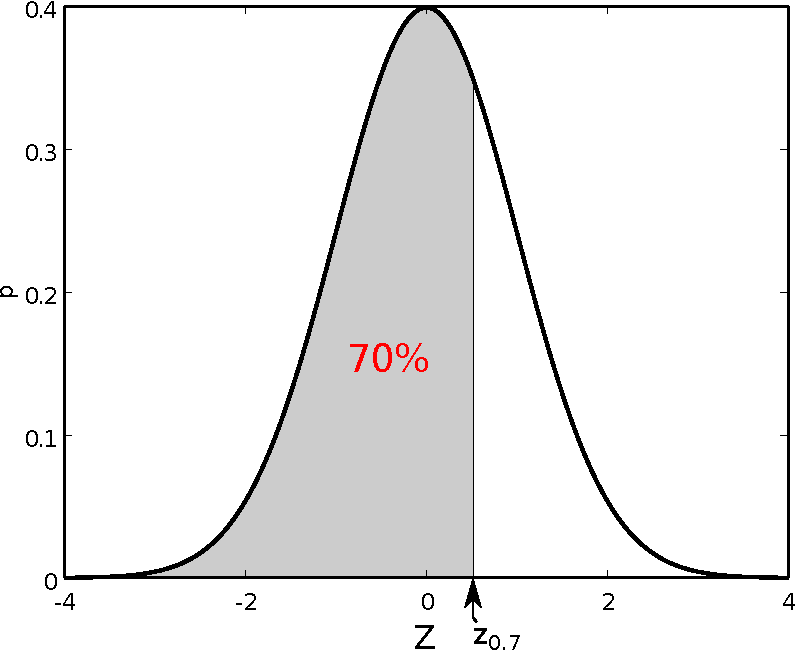
\includegraphics[width=79mm]{05_vorlesung/media/normpdfQuantil.pdf}
\hspace{5mm}
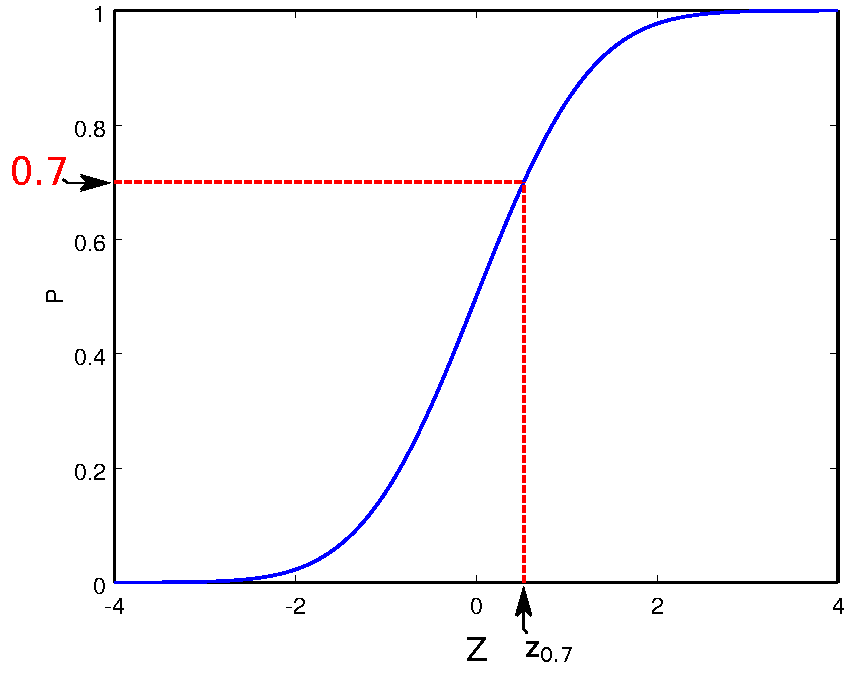
\includegraphics[width=81mm]{05_vorlesung/media/normcdfQuantil.pdf}
\caption{\label{normVertQuantil} Quantil $z_\alpha = 0.5244$ und Wahrscheinlichkeit
$\alpha = 0.7$ der Standard\-normalverteilung.}
\end{center}
\end{figure}

Dies lesen wir so:
\begin{quote}
Die Ereignisse Werte zu $Z$ zu beobachten, die kleiner sind als $z_\alpha$, können
mit einer Wahrscheinlichkeit von $\alpha$ eintreten.
\end{quote}
Die in den Tabellenwerken gelisteten Wahrscheinlichkeiten $\alpha$ werden
aus der Integration der Wahrscheinlichkeitsdichte der normierten Zufallsgröße
von minus Unendlich bis zu einer endlichen oberen Integrationsgrenze $z_\alpha$
gewonnen.
Die zu einem Wert eines Quantils gehörende Wahrscheinlichkeit wird durch den tiefgestellten
Index bei $z_\alpha$ gekennzeichnet, in unserem Beispiel aus Abb.~\ref{normVertQuantil}
ist dies dann
$$
z_{0.7} \; = \; 0.5244
$$
Als weiteres Beispiel betrachten wir die Frage, wie hoch die Wahrscheinlichkeit ist,
Werte zu beobachten, die in den Ausläufern einer Verteilungsdichte liegen.
Die Ausläufer werden im Englischen
als \textsl{Tails} (Schwänze) bezeichnet. Dies sollen Beobachtungen zu der normierten
Zufallsgröße $Z$ mit Werten, die zum einen kleiner oder gleich $-1.960$ sind, sein
$$
z_{0.025} \; = \; -1.960
$$
und zum anderen, die Beobachtungen mit Werten größer oder gleich $1.960$, also die
in dem rechten Ausläufer (\textsl{Tail}) der Standardnormalverteilung liegen.
Die Wahrscheinlichkeit für Beobachtungen im linken \textsl{Tail} ist
\begin{equation*}
\int\limits_{-\infty}^{-1.960} p(Z) \mathrm{d} Z \; = \; 0.025 .
\end{equation*}

Aufgrund der Symmetrie der Standardnormalverteilung ist die Wahrscheinlichkeit für das Liegen von
Werten im rechten \textsl{Tail} ebenfalls $0.025$. Wir rechnen also zusammen, dass mit
einer Wahrscheinlichkeit von $0.05 = 0.025+0.025$ Werte in den beiden \textsl{Tails} außerhalb
des Intervalls $[-1.960, 1.960]$ liegen können. Somit ist die Wahrscheinlichkeit, dass sie
innerhalb des Intervalls liegen $1 - 0.05 = 0.95$
\begin{equation}
\int\limits_{-1.96}^{1.96} \, p(Z) \, \operatorname{d} Z \; = \; 0.95
\end{equation}
was uns zeigt, wie wir die Tabellen zu verwenden haben.
Wenn wir ein zweiseitiges Intervall betrachten wollen, wie hier zu einem Vertrauensniveau
von $95 \%$, so müssen wir im Tabellenwerk nach dem Quantil, das für $97.5 \%$ gelistet
ist, schauen
$$
z_{0.975} \; = \; 1.960
$$
weil
$$
0.95 \; = \;
\underbrace{\int\limits_{-\infty}^{z_{0.975}} \, p(Z) \, \operatorname{d} Z}_{0.975} \; - \;
\underbrace{\int\limits_{-\infty}^{z_{0.025}} \, p(Z) \, \operatorname{d} Z}_{0.025}
$$
Aufgrund der Achssymmetrie der Normalverteilung gilt
$$
z_{\frac{1}{2}\alpha} = -z_{1-\frac{1}{2}\alpha} .
$$
Da sich die Quantile zum jeweiligen Vertrauensniveau $1-\alpha$ auf die normierte Zufallsgröße
beziehen, muss für die Berechnung des Vertrauensintervalls zurückgerechnet werden
\begin{equation}
Z \; = \; \frac{X - \mu}{\sigma} \qquad \Leftrightarrow \qquad X \; = \; \mu + Z \sigma
\end{equation}
also
\begin{equation}
[z_{\frac{1}{2}\alpha}, z_{1-\frac{1}{2}\alpha}] =
[-z_{1-\frac{1}{2}\alpha}, z_{1-\frac{1}{2}\alpha}]
 \qquad \Leftrightarrow  \qquad
[\mu \, - \, z_{1-\frac{1}{2}\alpha} \, \sigma, \mu \, + \, z_{1-\frac{1}{2}\alpha} \, \sigma]
\end{equation}
Mit $\alpha$ sind die $5 \%$ Signifikanzniveau und mit $1-\alpha$ die $95 \%$ Vertrauensniveau gemeint.

Die Likelihood wird maximal für
\begin{equation}
y \; = \; \frac{1}{J} \sum_{j=1}^J X_{1,j} ,
\end{equation}
wobei $y$ der Schätzwert für den Modellparameter $Y$ ist.
Der Schätzwert $s^2$ für die Varianz $\sigma^2$ wird berechnet mit
\begin{equation}
s^2 \; = \; \frac{1}{J-1} \sum_{j=1}^J (X_{1,j} - y)^2 .
\end{equation}

\section{Konzept der bayesischen Verfahren zum Lösen inverser Probleme}
\label{bayeskonzept}

Für komplexere Fragestellungen hinsichtlich der Varianzen und hinsichtlich der Möglichkeit,
sukzessive neue Informationen durch weitere Beobachtungen zu bereits geschätzten Modellparametern
hinzuzufügen und damit die Werte von
interessierenden indirekten Messgrößen immer weiter zu verbessern, stoßen die gängigen Ansätze
der Maximum-Likelihood-Methode an gewisse Grenzen. Insbesondere die Möglichkeit, bereits durch
vergangene Optimierungsprozesse gewonnene Parameter durch Gewinnen neuer Beobachtungen zu verändern,
ist nicht Gegenstand der \glqq herkömmlichen\grqq ~Statistik. Mit \glqq herkömmlich\grqq ~ist
an dieser Stelle die \textsl{frequentistische} Statistik gemeint, bei der empirisch aus
Beobachtungen Häufigkeitsverteilungen gewonnen werden, empirische Wahrscheinlichkeitsverteilungen
(Likelihood) berechnet werden, und entsprechend eine Schätzung von Modellparametern erfolgt.
Die lineare Regression ist ein Teilgebiet der \textsl{frequentistischen} Statistik

In der Statistik gibt es dazu zweierlei Blickrichtungen:
\begin{enumerate}
\item In der \textbf{frequentistischen Statistik} wird angenommen,
dass der Wert einer indirekten Messgröße unbekannt, aber konstant/ fest ist und deshalb
auch \textsl{wahrer Wert} genannt wird. In Bezug auf die direkt messbaren Größen wird angenommen,
dass sie aufgrund des Mangels an Erkenntnis über alle möglichen Einflüsse und Abläufe im Messprozess
streuen, so dass sie als Zufallsgrößen behandelt werden. Die Behandlung als Zufallsgröße
bedeutet dabei, dass der Wahrscheinlichkeit für eine Beobachtung einen konkreten Wert anzunehmen eine
Wahrscheinlichkeitsdichteverteilung zugrunde gelegt wird.
\begin{equation}
\underbrace{(Y_1, \dots, Y_M)}_{\mathrm{unbek, konst, wahr}} \xrightarrow{\mathrm{Messprozess}}
\underbrace{(X_1, \dots, X_N)}_{\mathrm{Zufallsgroessen}}
\end{equation}
\item Umgekehrt ist die Weise, wie das Zustandekommen der Streuung von Größen gesehen wird,
in der Statistik, die den Satz von Bayes zum Berechnen bedingter Wahrscheinlichkeiten
verwendet. Dieses Gebiet der Statistik wird wegen der Verwendung des
Satzes von Bayes auch \textbf{bayesische Statistik} genannt.

Hier werden die Beobachtungen der direkten Größen, als konkrete, feste Werte eingesetzt,
um die Erkenntnis über die zu bestimmende indirekte Größe zu überprüfen bzw.\ zu vermehren.
Die Vorstellung ist, dass durch den Mangel an Erkenntnis die indirekten Größen als
Zufallsgrößen zu behandeln sind. Es wird nun also nicht mehr nur eine Likelihood-Verteilung
berechnet, deren Maximum gesucht wird. Sondern es wird eine Kombination der Likelihood mit
einer Wahrscheinlichkeitsdichteverteilung,
die eine {\`a} priori Annahme über die indirekten Messgrößen darstellt, berechnet und der
Erwartungswert (das erste statistische Moment) und die Varianz (das zweite statistische Moment)
dieser kombinierten Verteilungsdichte ermittelt.

Dabei repräsentieren die Wahrscheinlichkeiten für die zu erwartenden Beobachtungen eines Parameters
(einer indirekten Messgröße),
den Grad der Erkenntnis, vernünftiger Glaubwürdigkeit, über die indirekte Messgröße.
In der englischsprachigen Literatur wird dies \textsl{Degree of Belief} genannt.

Vielleicht kann man sich diese Denkweise so vorstellen wie die Vorgehensweise eines Detektivs
oder Kriminalkommissars beim Sammeln von immer mehr Indizien zum Aufklären eines Falls.
\begin{equation}
\underbrace{(X_1, \dots, X_N)}_{\mathrm{Beobachtungen}} \xrightarrow{\mathrm{inverses \; Problem}}
\underbrace{(Y_1, \dots, Y_M)}_{\mathrm{Zufallsgroessen}}
\end{equation}
Die Erkenntnis über die indirekten Größen (Modellparameter $Y_1, \dots, Y_M$) wird mit jeder
neuen Messkampagne $\kappa$ revidiert
\begin{equation}
\arraycolsep=2.4pt\def\arraystretch{2}
\left.
\begin{array}{l}
\underbrace{(X_1, \dots, X_N)}_{\mathrm{neue~Beobachtungen}}\\
\underbrace{(Y_1, \dots, Y_M)_{\kappa-1}}_{\mathrm{Zufallsgroessen, vorher}}
\end{array}\right\}
 \xrightarrow{\mathrm{inverses \; Problem}}
\underbrace{(Y_1, \dots, Y_M)_{\kappa}}_{\mathrm{Zufallsgroessen}}
\end{equation}
\end{enumerate}
Da wir wie vorher detailiert dargelegt die indirekten Größen durch approximative Modellparameter ersetzten,
also $Y_m \approx P_m$, sind es die Schätzungen zu den Parametern $\mathbf{p} = (P_1,\dots,P_M)$, die
sozusagen \glqq\textsl{upgedated}\grqq ~werden.
\begin{equation}
\arraycolsep=2.4pt\def\arraystretch{2}
\left.
\begin{array}{l}
\underbrace{(X_1, \dots, X_N)}_{\mathrm{neue~Beobachtung}}\\
\underbrace{(P_1, \sigma^2_1, \dots, P_M, \sigma^2_M)_{\kappa-1}}_{\mathrm{Zufallsgroesse, vorher}}
\end{array}\right\}
 \xrightarrow{\mathrm{inverses \; Problem}}
\underbrace{(P_1, \sigma^2_1, \dots, P_M, \sigma^2_M)_{\kappa}}_{\mathrm{Zufallsgroesse}}
\end{equation}

Die hier umgangsprachlich einfach \glqq\textsl{updaten}\grqq ~der Modellparameter genannte
Veränderung der Parameter aufgrund neuer Beobachtungen, das heißt neuer Informationen, wird
Informationszuwachs oder Erkenntniszuwachs genannt. In Abb.\ \ref{BayesFreqVergleich}
sind die beiden Heransgehensweisen der frequentistischen und der bayesischen Statistik im
Überblick dargestellt.

\begin{figure}
\begin{center}
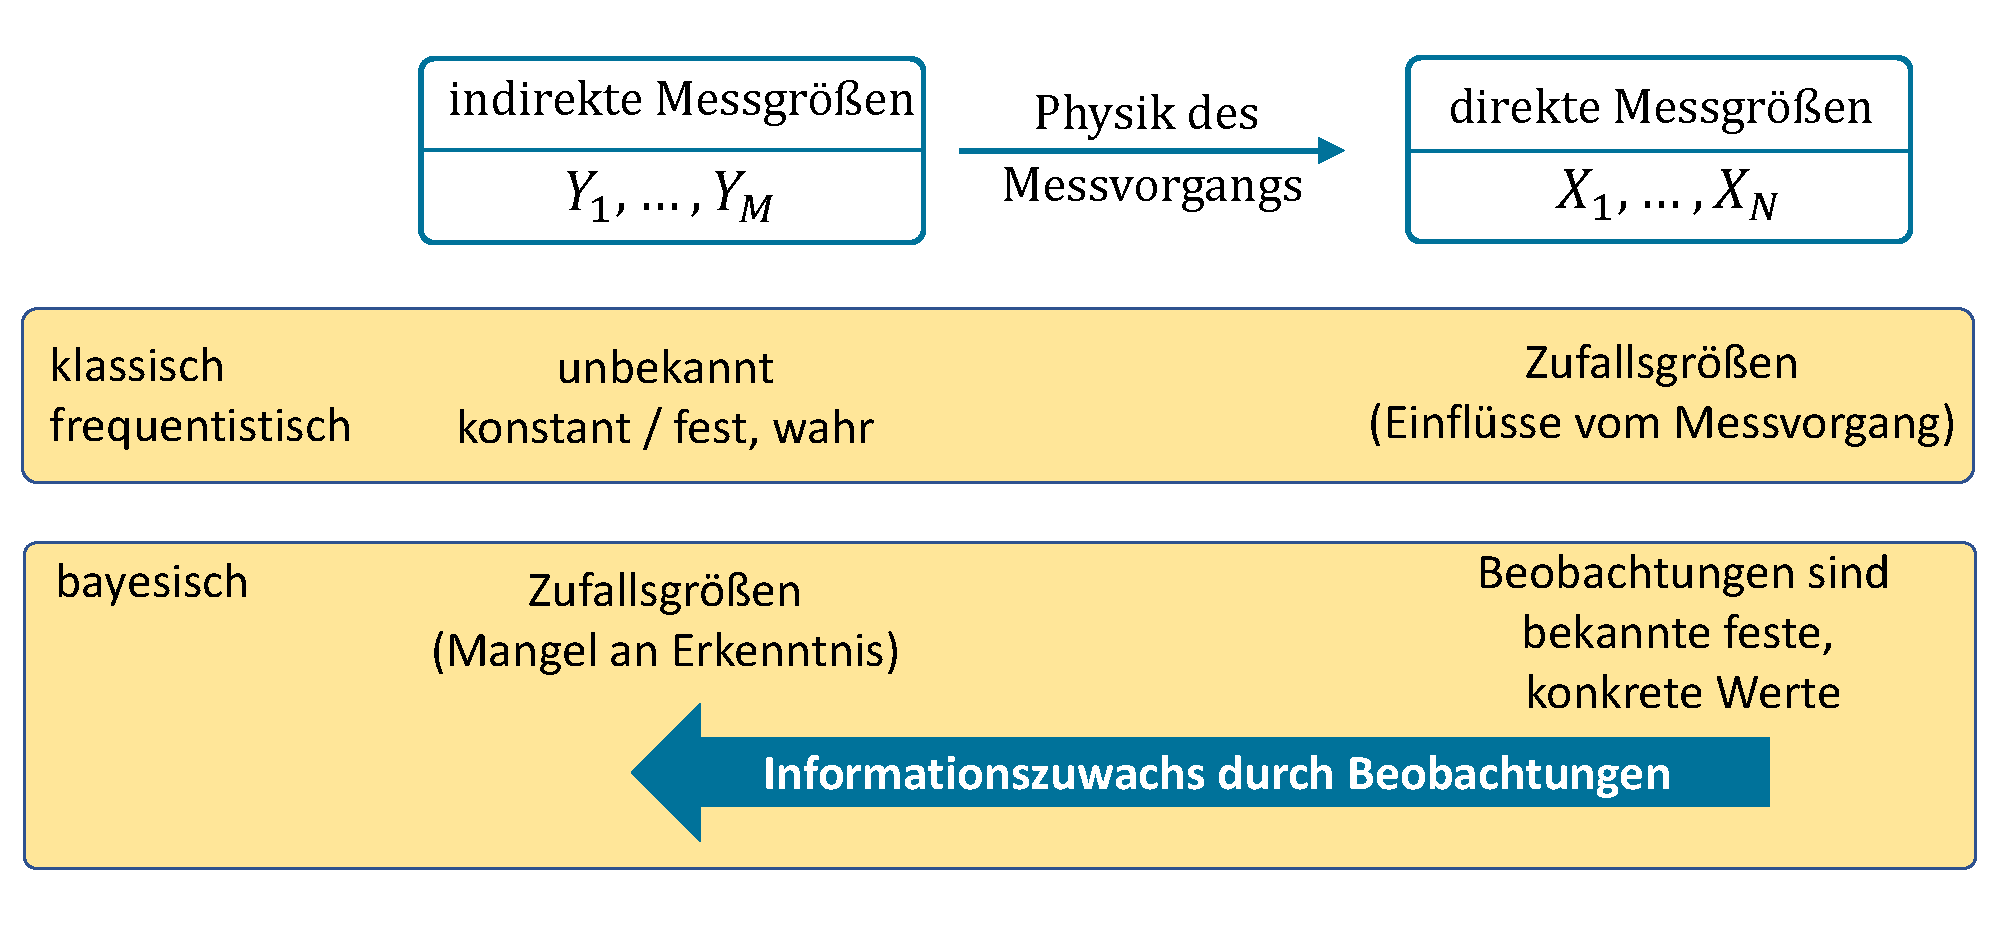
\includegraphics[width=140mm]{04_vorlesung/media/Konzept_Bayes.pdf}
\caption{Übersicht zu den Heransgehensweisen der frequentistischen und der bayesischen
Statistik}
\label{BayesFreqVergleich}
\end{center}
\end{figure}

Der Heransgehensweise, einen Informationszuwachs statistisch zu verarbeiten, liegt der \textsl{Satz von
Bayes} zu bedingten Wahrscheinlichkeiten zugrunde:
\begin{equation}
p(M | D) \; = \; \frac{p(D | M) p(T)}{p(D | M) p(M) \, + \, p(D | \lnot M) p(\lnot M)}
\label{bayestheorem}
\end{equation}
mit $M$ für die Theorie und $D$ für die Indizien (engl.\ \textsl{evidence}).


Die Theorie ist dabei
ein Modell $f$ mit Parametern $\mathbf{p}$, $\boldsymbol{\Sigma}$, die als statistisches Ereignis $M$
betrachtet wird. Die Indizien sind die Tupel von Beobachtungen zu
den direkten Messgrößen, die Daten, die ebenfalls als Ereignis $D$ betrachtet werden.
\begin{itemize}
\item $p(M)$ heißt \textsl{Prior}:

Wahrscheinlichkeit des {\`a} priori geschätzten
Modells mit $(\mathbf{p}_0, \boldsymbol{\Sigma}_0)$

\item $p(M | D)$ heißt \textsl{Posterior}:

Wahrscheinlichkeit des Modells mit Parametern $(\mathbf{p}, \boldsymbol{\Sigma})$
für die neuen Beobachtungen, also den hinzugewonnenen Datensatz
 $D = \{(X_{1,1},\dots,X_{1,J}), \dots,(X_{N,1},\dots  X_{N,J})\}$.
\end{itemize}

% ----------

Für das Verständnis, wie das Prinzip der bayesischen Statistik funktioniert,
betrachten wir das ganz einfache Beispiel Gl.~(\ref{oneQuantityOnly1}), also
 den einfachsten Fall einer einzigen Größe. Der Modellparameter $P = \mu$ repräsentiere
eine indirekte Messgröße $Y$. Die Größe $\mu$ ist aus einer Stichprobe zu schätzen.
Als {\`a} priori Information seien folgende Angaben bekannt:
\begin{itemize}
\item Der {\`a} priori Schätzwert der Modellgröße $\mu$ sei $y_0$.
\item Der {\`a} priori Schätzwert seiner Varianz $\sigma^2$ sei $s^2_0$.
\item Diese Größe sei normalverteilt, also verwenden wir als
Verteilungsdichtefunktion $p$ die Gaußverteilung.
\end{itemize}
Die neue Stichprobe $\{X_{1,1}, \dots, X_{1,J}\}$ sei vom Umfang deutlich kleiner als
die Informationsbasis, die dem {\`a} priori-Wissen zugrunde gelegen hat, so dass
für die Streuung der Varianz die $\chi^2$-Verteilung $p_{\chi^2,\nu}$
für $\nu = J-1$ Freiheitsgrade verwendet wird. Hierzu müssen wir im Stoff vorgreifen.
Diese Verteilungsdichtefunktion werden wir in der 5.\ Vorlesung behandeln.
Sie wird verwendet als Verteilungsdichte für Varianzen und ist eine schiefsymmetrische
Verteilung mit längerem Ausläufer zu größeren Werten. Je kleiner der Stichprobenumfang,
desto schiefer die Verteilung und ausgeprägter die Ausläufer.

Die gesamte Wahrscheinlichkeitsdichteverteilung $p(Y,\sigma)$ für die indirekte Messgröße
$Y$ bzw.\ deren Approximation als Modellparameter $P = \mu$ mit Streuung $\sigma$ wird als Produkt
folgender Wahrscheinlichkeiten berechnet,
\begin{itemize}
\item der Likelihood $p_\mathrm{L}$,
\item der Verteilungsdichte $p_\mathcal{N}(y | y_0, s_0)$ der Größe $\mu$ aus den {\`a} priori Informationen,
\item der Verteilungsdichte $p_{\chi^2,\nu}(s)$ der Varianz $\sigma^2$ dieser Größe.
\end{itemize}
Die zu ermittelnde bedingte Wahrscheinlichkeitsdichte wird so interpretiert, dass die Verteilung Funktion
der Variablen $\mu$ und $\sigma$ ist, gegeben die Beobachtungswerte der Stichprobe. Die Likelihood wird
dabei betrachtet als die bedingte Wahrscheinlichkeitsdichte $p_\mathrm{L}$ der
direkten Messgröße $X_1$ gegeben die Modellparameter $\mu$ und $\sigma$:
\begin{equation}
p_\mathrm{L}(\{X_{1,1}, \dots, X_{1,J}\} | \mu, \sigma) \; = \;
\prod\limits_{j=1}^J \frac{1}{\sqrt{2 \pi} \, \sigma}
 e^{- \frac{1}{2} \, \left( \frac{X_{1,j} - \mu}{\sigma} \right)^2 }  \; = \;
l(\mu, \sigma | \{X_{1,1}, \dots, X_{1,J}\}).
\end{equation}
Die Varianz $\sigma^2$ wird gemäß der $\chi^2$-Verteilung variiert. Das Variieren der Varianz
bzw.\ deren Wurzel $\sigma$ symbolisieren wir durch den Gebrauch der Variablen $s$.
Das Variieren des Modellparameters $\mu$ symbolisieren wir durch den Gebrauch der Variablen $y$.
Der Parameter $\mu$ wird ebenfalls variiert gemäß der Gaußverteilung, wir verwenden folgende
Likelihood:
\begin{equation}
p_\mathrm{L}(\{X_{1,1}, \dots, X_{1,J}\} | y, s) \; = \;
\prod\limits_{j=1}^J \frac{1}{\sqrt{2 \pi} \, s}
 e^{- \frac{1}{2} \, \left( \frac{X_{1,j} - y}{s} \right)^2 }  \; = \;
l(y, s | \{X_{1,1}, \dots, X_{1,J}\}).
\end{equation}

\begin{figure}
\begin{center}
\includegraphics[width=100mm]{04_vorlesung/media/understand_bayes_mean_posteriormatrix.pdf}
\caption{\label{posteriormatrix} Posterior-Wahrscheinlichkeitsdichte als Funktion
der beiden zu schätzenden Größen $y$ und $s$.}
\end{center}
\end{figure}
Das Produkt ist die Wahrscheinlichkeit des Modellparameters und dessen Varianz gegeben
die Stichprobe $\{X_{1,1}, \dots, X_{1,J}\}$ und die {\`a} priori Informationen $y_0, s_0$
\begin{equation}
p(y, s | \{X_{1,1}, \dots, X_{1,J}\}, y_0, s_0) \; = \; C \,
p_\mathrm{L}(\{X_{1,1}, \dots, X_{1,J}\} | y, s) \; p_\mathcal{N}(y | y_0, s_0) \; p_{\chi^2,\nu}(s)
\label{ProduktWahrscheinlichkeiten}
\end{equation}
mit $C$ als Normierungsfaktor derart zu wählen, dass die integrierte Wahrscheinlichkeit Eins ist, d.h.
$$
\int\limits_{-\infty}^\infty  \int\limits_0^\infty \; p(y, s | \{X_{1,1}, \dots, X_{1,J}\}, y_0, s_0) \;
\mathrm{d}s \, \mathrm{d}y \; = \; 1 .
$$
Die Verteilungsdichte $p(y, s | \{X_{1,1}, \dots, X_{1,J}\}, y_0, s_0)$ ist Funktion der
Variablen $y$ und $s$ mit vorgegebenen Parametern
(festen Werten) $\{X_{1,1}, \dots, X_{1,J}\}$, $y_0, s_0$, wie es beispielhaft in
Abb.~\ref{posteriormatrix} dargestellt wird.

Die Wahrscheinlichkeitsdichteverteilung
$p_\mathcal{N}(y | y_0, s_0)$ wird \textsl{Prior} genannt und die
Wahr\-schein\-lich\-keits\-dichte\-ver\-teilung $p(y, s | \{X_{1,1}, \dots, X_{1,J}\}, y_0, s_0)$
wird \textsl{Posterior} genannt.

Wir integrieren Gl.~(\ref{ProduktWahrscheinlichkeiten}) über $s$, um eine
Wahrscheinlichkeits\-dichte\-verteilung zu gewinnen, die nur noch Funktion von $y$ ist
\begin{equation}
p(y | \{X_{1,1}, \dots, X_{1,J}\}, y_0, s_0)  \; = \;
\int\limits_0^\infty p(y, s | \{X_{1,1}, \dots, X_{1,J}\}, y_0, s_0) \operatorname{d}s
\label{RandverteilungPosterior}
\end{equation}
Diese Verteilung wird \textsl{Randverteilung} oder \textsl{Marginalverteilung} genannt.
Allgemeiner gilt: Gegeben zwei Zufallsgrößen $A$ und $B$ mit gemeinsamer Verteilungsdichte
$p(A, B)$; dann heißen die Verteilungen der einzelnen Zufallsgrößen
$A$ und $B$ die Randverteilungen des Zufallsvektors $(A, B)$.

Als Schätzwert für $Y$ berechnen wir den Erwartungswert des Modellparameters $\mu$
durch Integration über alle Werte $y$ gewichtet mit der Wahrscheinlichkeitsdichte
$p(y | \{X_{1,1}, \dots, X_{1,J}\}, y_0, s_0)$ aus Gl.~(\ref{RandverteilungPosterior})
\begin{equation}
y_1 \; = \; \int\limits_{-\infty}^\infty \, y \, p(y | \{X_{1,1}, \dots, X_{1,J}\}, y_0, s_0)
\operatorname{d}y
\end{equation}
wobei wir $y_1$ mit Index $1$ schreiben, um anzuzeigen, dass dies die Revision der Schätzung des
Modellparameters $\mu \approx Y$ gegenüber vorheriger Kenntnis mit Schätzwert $y_0$ ist.

Wir rufen uns die Definition des vollständigen Messergebnisses in Erinnerung, das aus
dem Schätzwert einer Messgröße und den beigeordneten Informationen, die entweder
direkt die Wahrscheinlichkeitsdichteverteilung sein kann oder aber, im Falle einer
symmetrischen Verteilung, deren Breite und das Vertrauensniveau.

Die als beigeordnete Information gegebene Wahrscheinlichkeitsdichteverteilungen sind
die in den Gln. (\ref{Likelihood2}) und (\ref{LikelihoodKov2}) vorgestellen Likelihoods oder
der in Gl.~(\ref{RandverteilungPosterior}) vorgestellten Posterior
mit gemeint:
$$
p(y | \{X_{1,1}, \dots, X_{1,J}\}, y_0, s_0)
$$
Die Likelihood wird
für kleine Stich\-proben\-um\-fänge ($N < 100$) anstelle durch eine Gaußverteilung durch eine Verteilung
repräsentiert, deren Charakteristik im Kurvenverlauf
überhöhter und mit länger auslaufenden Rändern ist. Sie wird $t$-Verteilung genannt.
Wir werden später in Kapitel \ref{wahrscheinlichHyp} auf diesen Verteilungtyp zurück kommen.

Allgemein betrachten wir für beide Fälle eine Wahrscheinlichkeitsdichtefunktion $p \! : y \mapsto p(y)$.
Der Definitionsbereich für $y$ reicht von minus bis plus Unendlich. Von Interesse ist der Kernbereich
der Dichteverteilung für eine spezifizierte Wahrscheinlichkeit $1-\alpha$, beispielsweise
$1-\alpha = 0.95$ oder $0.90$ oder so.
Dies ist die Wahrscheinlichkeit einer Größe, einen Messwert im Bereich (Intervall) $[y_\mathrm{min}, y_\mathrm{max}]$,
anzunehmen
\begin{equation}
1 \, - \, \alpha \; = \;
\int\limits_{y_\mathrm{min}}^{y_\mathrm{max}} p(y)
\operatorname{d}y .
\label{UeberdeckungWahrscheinlichkeit}
\end{equation}
Die Breite des Intervalls gibt dann die \textsl{Messunsicherheit} an.

Das Intervall $[y_\mathrm{min}, y_\mathrm{max}]$, zu dem die Fläche $1 - \alpha$ unter der die
Verteilungsdichte $p(y)$ repräsentierenden Kurve gehört, wird \textsl{Überdeckungsintervall} genannt.
Es ist der verallgemeinerte Begriff aus der Metrologie für das, was in der
\textsl{frequentistischen} Statistik \textsl{Vertrauensintervall},
engl.\  \textsl{Confidence Interval}, und in der \textsl{bayesischen} Statistik
\textsl{Glaubwürdigkeitsintervall}, engl.\ \textsl{Credible Interval},
heißt. Während der Begriff \textsl{Vertrauensintervall} in der deutschsprachigen
Literatur üblich ist, wird anstelle des Begriffs \textsl{Glaubwürdigkeitsintervall} üblicherweise
auch in der deutschsprachigen Literatur der Begriff \textsl{Credible Interval} verwendet.

Die Verwendung unterschiedlicher Bezeichnungen, \textsl{Confidence Interval} und
\textsl{Credible Interval}, soll die Unterschiedlichkeit der Vorstellungen
über den Charakter einer indirekten Messgröße $Y$ zum Ausdruck bringen.
Die Unterschiedlichkeit in der Vorstellung von einer indirekten Messgröße $Y$ besteht darin,
dass im Fall der \textsl{bayesischen} Statistik
die indirekte Messgröße $Y$ als Größe, die intrinsisch eine Zufallsgröße ist, betrachtet
wird. Im Fall der \textsl{frequentistischen} Statistik wird $Y$ als eine Größe betrachtet,
die einen festen, wahren Wert hat, der aber nicht zugänglich ist. Nur der
Modellparameter, der eine indirekte Messgröße approximiert und der indirekt aus anderen
Zufallsgrößen gewonnen wird, wird als daraus resultierend einer Streuung unterliegend betrachtet.

Die Wahrscheinlichkeit $1 - \alpha$ wird in der \textsl{frequentistischen} Statistik
\textsl{Vertrauensniveau} genannt. Die beiden Flächen unter den
Ausläufern der Dichteverteilung stellt eine Wahrscheinlichkeit $\alpha$ dar, die in der
\textsl{frequentistischen} Statistik \textsl{Signifikanzniveau} genannt wird.

Im folgenden werden wir sehen, wie eine \textsl{Messunsicherheit} im Rahmen der
\textsl{bayesischen} Statistik gewonnen wird.
Die Grenzen des \textsl{Credible Interval} $[y_\mathrm{min}, y_\mathrm{max}]$ bilden die
Integrationsgrenzen $y_\mathrm{min}$ und $y_\mathrm{max}$ der \textsl{Posterior}, so dass
\begin{equation}
1 \, - \, \alpha \; = \;
\int\limits_{y_\mathrm{min}}^{y_\mathrm{max}} p(y | \{X_{1,1}, \dots, X_{1,J}\}, y_0, s_0)
\operatorname{d}y .
\label{UeberdeckungPosterior}
\end{equation}
Die Integrationsgrenzen werden über die Umkehrfunktion der kumulativen Verteilung $P$ berechnet.
Die kumulative Verteilung $P$ ist
\begin{equation}
P(y) \; = \; \int\limits_{-\infty}^{y} p(y^\prime | \{X_{1,1}, \dots, X_{1,J}\}, y_0, s_0)
\operatorname{d}y^\prime .
\end{equation}
Die Umkehrfunktion schreiben wir symbolisch als $P^{-1}$.
Wir berechnen für das \textsl{Credible Interval}
\begin{equation}
y_\mathrm{min} \, = \, P^{-1}(\frac{\alpha}{2}) \qquad \mathrm{und} \qquad
y_\mathrm{max} \, = \, P^{-1}(\frac{1-\alpha}{2}).
\end{equation}
\begin{figure}
\begin{center}
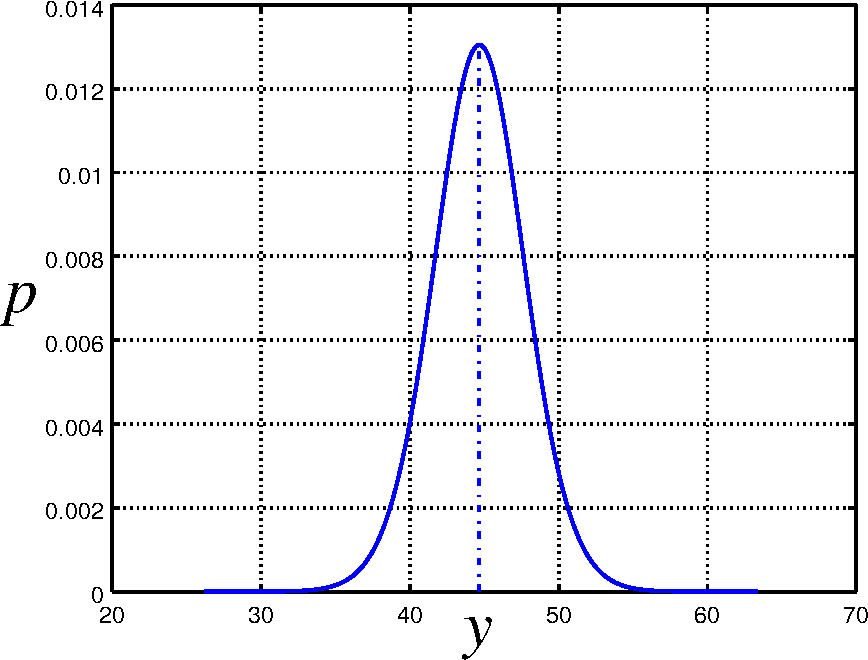
\includegraphics[width=80mm]{04_vorlesung/media/understand_bayes_mean_posteriormarginal.pdf}
\hspace{5mm}
\includegraphics[width=80mm]{04_vorlesung/media/understand_bayes_mean_cumposterior.pdf}
\caption{\label{posteriorCredible}\textsl{Links:} Die blaue Kurve stellt die
Randverteilung der Posterior-Wahrscheinlichkeitsdichte als Funktion
der beiden zu schätzenden Größen $Y$ mit \textsl{Credible Interval} dar und die
rot gestrichelte Kurve die Student-t-Verteilung mit Vertrauensintervall.
\textsl{Rechts:} Kumulierte Randverteilung der Posterior-Wahrscheinlichkeitsdichte, deren
Umkehrfunktion verwendet wird, um die Intervallgrenzen des \textsl{Credible Interval}s zu ermitteln.}
\end{center}
\end{figure}
Abb.~\ref{posteriorCredible} links zeigt im Vergleich folgende Verteilungsdichten
\begin{itemize}
\item die Posterior als Funktion des Parameters
$y$ mit einem \textsl{Credible Interval} für eine Wahrscheinlichkeit von
$1 - \alpha = 0.95$ (blaue, durchgezogene Kurve und blaue, durchgezogene Linien)
\item die $t$-Verteilung (rote, gestrichelte Kurve), die sich für die in dem
graphisch dargestellten Beispiel verwendeten Stichprobe mit Stichprobenumfang $J = 7$, folglich
$\nu = J - 1 = 6$ Freiheitsgraden ergeben hat, sowie das Vertrauensintervall (rote, gestrichelte Linien),
das aus dem Mittelwert der Stichprobe
und der empirischen Standardabweichung des Mittelwerts multipliziert mit dem
$t$-Quantil gewonnen wurde. Mit dem Begriff $t$-Quantil werden die Integrationsgrenzen dieser Verteilung
zu vorgegebenen Wahrscheinlichkeiten $\frac{\alpha}{2}$ und $1 - \frac{\alpha}{2}$ bezeichnet.
\end{itemize}

Abb.~\ref{posteriorCredible} rechts zeigt die kumulierte Posterior, aus deren Umkehrfunktion
zu den Wahrscheinlichkeiten $\frac{\alpha}{2}$ und $1 - \frac{\alpha}{2}$ die
Intervallgrenzen des \textsl{Credible Interval}s gewonnen werden.

Die Ermittlung der \textsl{Messunsicherheit} im Rahmen der
\textsl{frequentistischen} Statistik unter Verwendung der $t$-Verteilung
wird in den kommenden Wochen detailiert und mit Beispielen dargelegt werden.
Sie wird einen großen Teil dieser Vorlesungsreihe ausmachen und Klausurrelevanz haben.
